% !TeX program = xelatex
% !TeX encoding = utf8
% !TeX root = Analysis3.tex

%% TODO: publish to CTAN
\documentclass[margin=normal]{tex/hsrzf}

%%%%%%%%%%%%%%%%%%%%%%%%%%%%%%%%%%%%%%%%%%%%%%%%%%%
% Packages

%% TODO: publish to CTAN
\usepackage{tex/hsrstud}
\usepackage{tex/docstyle}

%% Language configuration
\usepackage{polyglossia}
\setdefaultlanguage{english}
% \setdefaultlanguage[variant=swiss]{german}

%% License configuration
\usepackage[
    type={CC},
    modifier={by-nc-sa},
    version={4.0},
]{doclicense}

%%%%%%%%%%%%%%%%%%%%%%%%%%%%%%%%%%%%%%%%%%%%%%%%%%%
% Metadata

\course{Electrical Engineering and Information Technology}
\module{Analysis3}
\semester{Fall 2022}

\authoremail{npross@student.ethz.ch}
\author{\textsl{Naoki Sean Pross} -- \texttt{\theauthoremail}}

% did someone help you with this work?
\contributors{
  % I created this template, does that count?
  Naoki Pross
  % do not forget to add yourself!
}

\title{Analysis 3 Notes}
\date{\thesemester}

%%%%%%%%%%%%%%%%%%%%%%%%%%%%%%%%%%%%%%%%%%%%%%%%%%%
% Document

\begin{document}

% use roman numberals for introductiory pages
\pagenumbering{roman}

\maketitle

\begin{abstract}
  These are my very unrigorous notes of the course Analysis 3 by Prof. Dr.
  Iacobelli at ETH Zürich. The content of this document was taken mostly from
  the lectures notes of Dr. Iacobelli, but sometimes also from the book
  ``\textsl{Introduction to Partial Differential Equations}'' by Peter J. Oliver
  (ISBN: \texttt{978-3-319-02098-3}).
\end{abstract}

% show the names of the people who contributed to this document.
% \section*{Contributors}
% \thecontributors

\section*{License}
\doclicenseThis

\tableofcontents


% actual content
\clearpage
\twocolumn 
\setcounter{page}{1}
\pagenumbering{arabic}

% vim: ts=2 sw=2 et tw=78:
\section{PDE and Cauchy Problems}

\begin{defn}[Linear PDE]
  A PDE is \emph{linear} if it has the form
  \[
    a_0 u + \sum_{i} a_{1,i} u_{x_i}
    + \sum_{i,j} a_{2,i,j} u_{x_i x_j}
    + \cdots = f(\mathbf{x})
  \]
\end{defn}

\begin{defn}[Quasilinear PDE]
  A PDE is said to be \emph{quasilienar} if it is linear in its highet
  derivatives.
\end{defn}

\begin{defn}[Strong or classical solution]
  A solution to a PDE is said to beh \emph{strong} or classical if all
  of its derivatives exist and are continuous.
\end{defn}

\begin{defn}[2D Cauchy problem]
  \label{def:cauchy-2d}
  In 2 dimensions a \emph{Cauchy problem} has the form
  \begin{equation}
    \label{eqn:cauchy-2d}
    \begin{cases}
      a u_x  + bu_y = c \\
      u(x_0, y_0) = u_0(x_0, y_0)
    \end{cases}
  \end{equation}
  where $a, b, c$ may be functions of $x, y$ and $u$.
\end{defn}



% vim: ts=2 sw=2 et tw=78:

\section{Method of Characteristics}

The method of charactersitics can be used to solve Cauchy problems with first
order quasilinear PDEs.

\subsection{General Case}

Suppose we have an $u(x,y)$ and let $x$ and $y$ be parametrized by a new
variable $t$, i.e. $x(t)$ and $y(t)$. Then if we take the derivative by the
chain rule:
\[
  \frac{d}{dt} u(x,y) = \frac{\partial u}{\partial x} \frac{dx}{dt}
    + \frac{\partial u}{\partial y} \frac{dy}{dt}.
\]
By comparing this to the general form we see that if we let
\[
  a(x,y,u,t) = \frac{dx}{dt}, \quad
  b(x,y,u,t) = \frac{dy}{dt},
\]
we obtain the left side of the general PDE of the Cauchy problem
\eqref{eqn:cauchy-2d}. Considering the right side we also have that $du/dt =
c$. Solving this system of ODEs for the functions $x(t)$, $y(t)$ and $u(t)$ is
equivalent to solving the PDE. Each ODE will yield an expression in $t$ and
each will have an integration constant. The solution to the PDE can only
depend on these integration constant which are found using the initial datum.

\begin{figure}
  \centering
  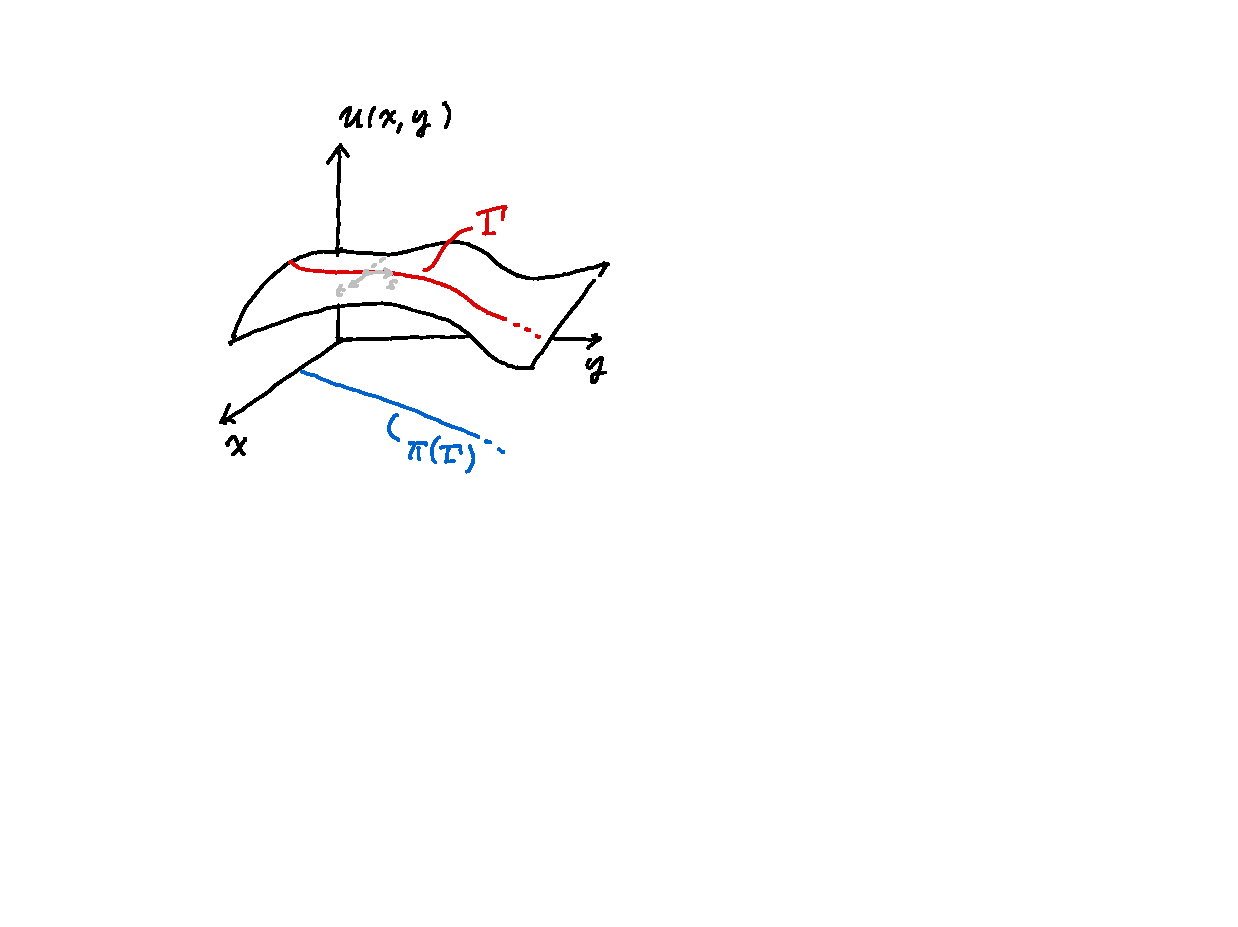
\includegraphics[
    width=.9\linewidth,
    trim=80 200 280 20, clip
  ]{figures/parametrization}
  \caption{
    Parametrization of the initial curve $\Gamma$ and its projection on the
    domain $\pi(\Gamma)$.
  }
\end{figure}

We parametrize the initial datum as a parametric curve $\Gamma$ with a
variable $s$, i.e.
\[
  \Gamma = \left\{
    \bigr( (x_0(s), y_0(s), u_0(s) \bigl) : s \in \mathbb{R}
  \right\}.
\]
For example if the initial curve is given as $u(x, 0) = x^2$, a good
parametrization is $\Gamma = \{ (s, 0, s^2) \}$. Then, these parametrization
are the initial values for the system of ODEs:
\[
  x(0) = x_0(s), \quad
  y(0) = y_0(s), \quad
  u(0) = u_0(s).
\]

Thus at the end of this process we have a solution $u$ to the PDE which is a
function of $(s, t)$; a local coordinate system. To conclude, we need to go
back to $(x,y)$, so we must invert the map to find $(s, t) \to (x(s,t),
y(s,t))$. This inversion is not always possible, to check whether the map is
(locally) invertible we use the \emph{transversality condition}.
\begin{thm}[Transversality condition]
  If the determinant of the Jacobian of a 2D Cauchy problem
  \[
    \det\begin{bmatrix}
      \partial_t x & \partial_t y \\
      \partial_s x_0 & \partial_s y_0
    \end{bmatrix}
    =
    \det\begin{bmatrix}
      a & b \\ \partial_s x_0 & \partial_s y_0
    \end{bmatrix}
    \neq 0,
  \]
  then there is a unique solution.
\end{thm}


\subsection{Special Cases}

If in \eqref{eqn:cauchy-2d} both $a$ and $b$ do \emph{not} depend on $u$ and
the PDE is homogeneous ($c = 0$) we can skip the parametrization. The PDE can
be rewritten using the dot product as
\[
  \begin{bmatrix} a(x,y) & b(x,y) \end{bmatrix}
    \cdot \nabla u(x,y) = 0,
\]
which is a directional derivative. With this interpretation we are saying that
$u$ must be constant along a curve defined by $a$ and $b$, which is equivalent
to stating that the slope must be given by
\[
  \frac{dy}{dx} = \frac{b(x,y)}{a(x,y)}.
\]
By solving this ODE we find the charactestic curves of $u$, one for each value
of the integration constant $k$. Thus the PDE has a general solution of the
form
\[
  u(x,y) = f(k(x,y)),
\]
and to find a particular solution one just needs to use the inital datum to
choose an appropriate $f$.

% vim: ts=2 sw=2 et tw=78 spell spelllang=en:
\section{Conservation Laws}

\begin{defn}[Conservation law]
  A \emph{conservation law} is a Cauchy problem of the form
  \begin{equation} \label{eqn:conservation-law}
    u_y + \partial_x f(u) = 0,
  \end{equation}
  for a given \emph{flux function} $f: \mathbb{R} \to \mathbb{R}$. An equivalent
  formulation is $u_y + c(u) u_x = 0$ with $c(u) = f'(u)$.
\end{defn}

\begin{defn}[Critical Time]
  Of an initial value (Cauchy) problem with conservation law
  \[
    \begin{cases}
      u_y + c(u) u_x = 0, & (x,y) \in \mathbb{R}\times(0,\infty), \\
      u(x, 0) = u_0(x), & x \in \mathbb{R},
    \end{cases}
  \]
  where $c, u_0 \in C^1(\mathbb{R})$ and such that $c \circ u_0 : \mathbb{R}
  \to \mathbb{R}$ is bounded and has bounded derivative, we interpret $y$ as
  being a ``time variable''. The \emph{critical time}
  \[
    y_c = \inf \left\{
      \frac{-1}{\alpha(s)}:
      s \in \mathbb{R}, \alpha(s) < 0
      \right\}
  \]
  where $\alpha(s) = \partial_s \bigl( c \circ u_0(s) \bigr) =
  c'(u_0(s))u_0'(s)$, is the time at which the solution is no longer smooth.
  If $\alpha(s) \geq 0$ for all $s \in \mathbb{R}$, we set by convention $y_c
  = \infty$.
\end{defn}
Therefore, the PDE has a unique solution in the interval $[0, y_c)$,
and $u$ satisfies the implicit equation
\[
  u(x,y) = u_0(x - c(u)y).
\]
Note that there can be multiple critical times, the infimum above only takes
the first. I.e. there could be a smooth solution solution after the critical
time, until a new critical time is reached.

\subsection{Weak solution}

\begin{defn}[Integral of a conservation law]
  Integrating \eqref{eqn:conservation-law} first wrt $x$ (space) then $y$
  (time) over an interval $X \times Y = [a,b)\times[y_1, y_2)$ results in
  \begin{align}
    \int_X u(x, y_2) &- u(x, y_1) \,dx \nonumber \\
    &= - \int_Y f(u(b,y)) - f(u(a,y)) \, dy.
    \label{eqn:conservation-law-int}
  \end{align}
\end{defn}

This is the \emph{integral formulation} of the conservation law, since if $u$
solves the conservation law \eqref{eqn:conservation-law} it also solves
\eqref{eqn:conservation-law-int}. However, because the integral is less
restrictive than the derivative and allows for discontinuities in the
solution, a solution to \eqref{eqn:conservation-law-int} may not be a solution
of \eqref{eqn:conservation-law}, it might be a \emph{weak solution}.

\begin{defn}[Weak solution and shocks]
  $u$ is a \emph{weak solution} on $D = \bigcup^n_{i=1} D_i$ if $u$ satisfies
  the PDE \eqref{eqn:conservation-law} in each $D_i$ for $i=1,\ldots,n$ and
  the integral form \eqref{eqn:conservation-law-int} on $D$. The boundaries
  between the regions $D_i$ are curves called \emph{shocks}.
\end{defn}

\begin{figure}
  \centering
  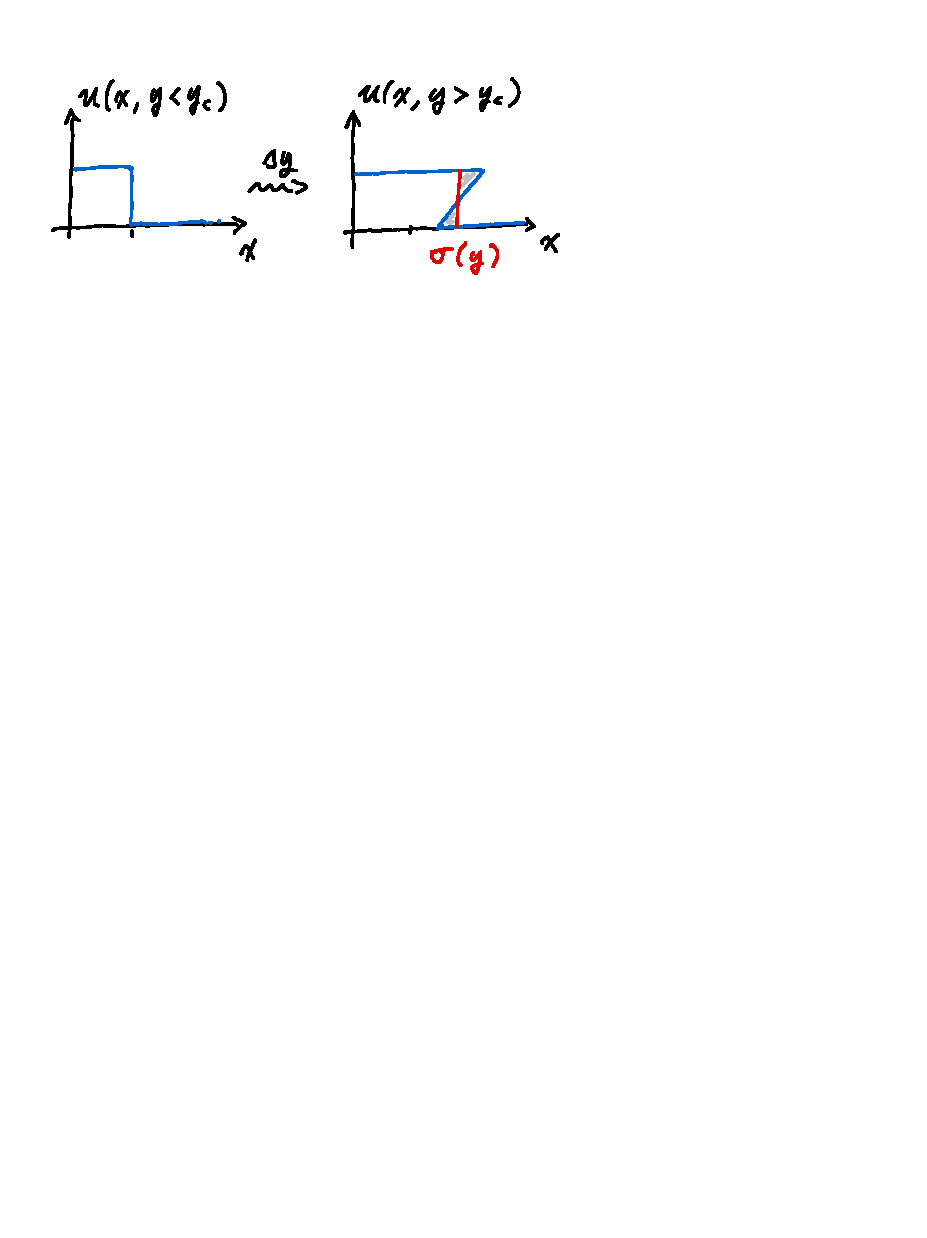
\includegraphics[
    width=.9\linewidth,
    trim=20 460 160 40, clip
  ]{figures/shockwave}
  \caption{
    \label{fig:shockwave}
    Shock wave. When the characteristic curves cross the function becomes
    multivalued. The multivalued region is replaced by a \emph{shock}
    $\sigma(y)$ which is placed such that the two gray regions have the same
    area.
  }
\end{figure}

Geometrically, the shocks are where the characteristic curves meet.
Intuitively this is a problem because the method of characteristics propagates
an information from the initial curve, and at the shock two different
information have propagated to that point (see Figure \ref{fig:shockwave}).

To check for the existence of a global weak solution, we enforce the
conservation of mass $M = \int_X u \,dx$ to the shock $\sigma(y)$, which
results in the following condition.

\begin{defn}[Ranikine-Huginot condition]
  For $u$ to be a solution weak solution of the conservation law
  \eqref{eqn:conservation-law} its \emph{shock waves} $\sigma(y)$ must have a
  speed of
  \[
    \frac{d\sigma}{dy} = \frac{f(u^+) - f(u^-)}{u^+ - u^-},
  \]
  where
  \[
    u^+(y) = \lim_{x \to\sigma(y)^+} u(x, y),
    \quad
    u^-(y) = \lim_{x \to\sigma(y)^-} u(x, y).
  \]
\end{defn}

The inverse problem to what lead to shock waves is when there is a region
where the characteristic curves \emph{diverge}, i.e. there are information to
propagate and the solution is undefined. There, the values would be
``created'' out of nothing and there are multiple solution that fit this
``hole''. Since PDEs model physical processes, a good choice is to fill in the
hole using a solution that does not break \emph{causality}, as imposed by the
next condition.

\begin{defn}[Entropy Condition]
  A weak solution satisfies the \emph{entropy condition} only if the
  characteristics enter the shock waves, and do not emerge from them. That is
  \[
    f(u^+) <
    \frac{d\sigma}{dy} = \frac{f(u^+) - f(u^-)}{u^+ - u^-}
    < f(u^-).
  \]
\end{defn}


% vim: ts=2 sw=2 et tw=78 spell:
\section{Second Order PDEs}

A second order PDE of two variables has in the most general case the form
\[
  Au_{tt} + Bu_{tx} + Cu_{xx} + Du_{t} + Eu_x + Fu = G.
\]
To classify them we define the \emph{discriminant}
\[
  \Delta = B^2 - 4AC,
\]
which is reminiscent of the quadratic equation. Now, the PDE is said to be
\begin{itemize}
  \item \emph{hyperbolic} if $\Delta(x,t) > 0$,
  \item \emph{parabolic} if $\Delta(x,t) = 0$ and $A^2 + B^2 + C^2 \neq 0$,
  \item \emph{elliptic} if $\Delta(x,t) < 0$,
  \item \emph{singular} if $A = B = C = 0$.
\end{itemize}
It is important to note that since the parameters may be function of $(x,t)$,
so is $\Delta(x,t)$ and the PDE may be different depending on where we are in
the domain. Some well known examples: the wave equation is hyperbolic, the
heat equation is parabolic and the Laplace equation is elliptic.

% vim: ts=2 sw=2 et tw=78 spell:

\section{Wave Equation}

\subsection{Homogeneous Case}

The homogeneous one dimensional wave equation is a linear second order
hyperbolic PDE:
\[
  u_{tt} - c^2 u_{xx} = 0
  \qquad (x, t) \in \mathbb{R} \times (0, \infty),
\]
where $c$ is to be interpreted as being a ``velocity''. To get an algebraic
intuition for the solution we can rewrite it as
\[
  (\partial_t - c\partial_x)(\partial_t + c\partial_x) u = 0,
\]
from which we can recognize the terms as transport equations and conclude that
the solutione are a linear combination of forward or backwards traveling
waves. The general solution to this problem can thus be written as
\begin{equation} \label{eqn:wave:solution}
  u(x,t) = p(\xi) + q(\eta)
\end{equation}
where the new variables are $\xi(x,t) = x - ct$ and $\eta(x,t) = x + ct$.
Note that by performing the change of variables to $(\xi,\eta)$ the wave
equation becomes $\partial_\xi \partial_\eta u = 0$.

\begin{defn}[Cauchy problem for the one dimensional wave equation]
  \label{def:wave:cauchy}
  \[
    \begin{cases}
      u_{tt} - c^2 u_{xx} = 0, & (x, t) \in \mathbb{R} \times (0, \infty), \\
      u(x,0) = f(x), \\
      u_t(x,0) = g(x).
    \end{cases}
  \]
\end{defn}

To solve the wave equation's Cauchy problem we assume that the has the form of 
\eqref{eqn:wave:solution}, so the two conditions become $u(x,0) = p(x) + q(x)
= f(x)$ and $\partial_t u(x,0) = -c p'(x) + c q'(x) = g(x)$. Solving for
$p(x)$ and $q(x)$ we get
\begin{align*}
  p(x) &= \frac{1}{2}f(x) - \frac{1}{2c}\int_0^x g(z) \, dz + a, \\
  q(x) &= f(x) - p(x) = \frac{1}{2}f(x) + \frac{1}{2c} \int_0^x g(z) \, dz -a,
\end{align*}
where $a$ is an integration constant. By combining the two and adding back the
time dependence we obtain d'Alambert's solution.
\begin{thm}[D'Alambert's solution]
  The solution to Cauchy problem of definition \ref{def:wave:cauchy} is given
  by
  \[
    u(x,t) = \frac{f(x-ct) + f(x+ct)}{2} 
      + \frac{1}{2c} \int_{x-ct}^{x+ct} g(z) \,dz.
  \]
\end{thm}

\subsection{Domain of influence and Characteristic Lines}

By inspecting d'Alambert's solution we should note that the solution only
depends on a wedge shaped region in the $(x,t)$ plane that starts at
$(f(x),0)$ and expands in time. The initial datum is propagated only in this
region between $x-ct$ and $x+ct$ that is known as the \emph{domain of
influence}. The aforementioned lines are the \emph{characteristic lines} of
the wave equation.

\subsection{Inhomogeneous Case}

In a more general setting the wave equation may be inhomogeneous, i.e. the
Cauchy problem is as follows.

\begin{defn}[Cauchy problem for the one dimensional inhomogeneous wave equation]
  \label{def:wave:inhom-cauchy}
  \[
    \begin{cases}
      u_{tt} =  c^2 u_{xx} + F(x,t), 
        & (x, t) \in\mathbb{R} \times (0, \infty), \\
      u(x,0) = 0, \\
      u_t(x,0) = 0.
    \end{cases}
  \]
\end{defn}

The initial conditions are set to zero for an easier solution, and their
effect can be added back later using superposition. To solve this case we also
use the change of coordinates to $(\xi,\eta) = (x-ct, x+tc)$. By the chain
rule the wave equation becomes
\[
  \frac{\partial^2 u}{\partial \xi \partial \eta}
  = -\frac{1}{4c^2} F\left(\frac{\eta - \xi}{2c}, \frac{\eta + \xi}{2c}\right).
\]
Integrating and using the fact that $\partial_\xi u(\xi,\xi) = 0$ because of
the zero initial conditions results in a double integral. After a change of
variables and making use of the superposition to add this solution to
d'Alambert's solution we obtain the following result.

\begin{thm}[D'Alambert's solution for the inhomogeneous wave equation]
  The solution to the general Cauchy problem of the inhomogeneous wave
  equation is given by
  \begin{align*}
    u(x,t) = &\frac{f(x-ct) + f(x+ct)}{2} 
      + \frac{1}{2c} \int_{x-ct}^{x+ct} g(z) \,dz \\
      &\quad + \frac{1}{2c}
        \int_0^t \int_{x+c(t-\tau)}^{x+c(t+\tau)} F(y, \tau) \, dy d\tau.
  \end{align*}
\end{thm}

A important observation is that the (double) integral is over a triangular
region $\Delta = \{ (y,\tau) : x - c(t - \tau) \leq y \leq c + c(t - \tau), 0
\leq \tau \leq t\}$ that is known as the \emph{domain of depence} of the wave
equation, since only the values in $F(\Delta)$ affect the solution.



\appendix

\section{ODEs and Initial Value Problems}

A recap on how to solve ODEs.

\subsection{First Order}



\end{document}
